\documentclass{article}


% Things to import:
\usepackage{tikz}
\usetikzlibrary{shapes.misc}


\begin{document}
% Used to export it as an image too: (Sourcecode is from here: https://tex.stackexchange.com/a/299008)
\hoffset=-1in\voffset=-1in\setbox0\vbox{

Example 1

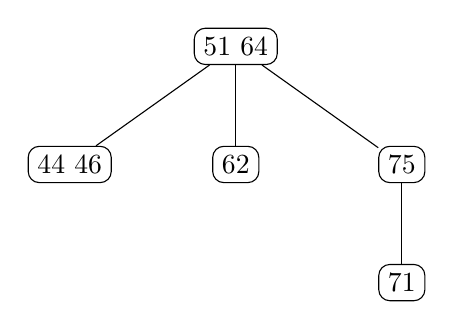
\begin{tikzpicture} [sibling distance=60, every node/.style = {shape=rectangle, rounded corners, draw, align=center}]
	\node (51 64){51 64}
	child { node (44 46){44 46}}
	child { node (62){62}}
	child { node (75){75}
		child { node (71){71}}
	};
\end{tikzpicture}
	
Example 2
	
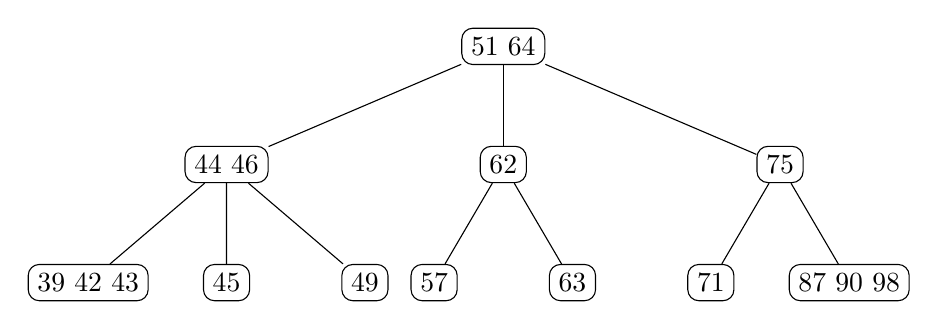
\begin{tikzpicture}[every node/.style ={shape=rectangle, rounded corners, draw, align=center}, sibling distance=100mm,level 1/.style={sibling distance=10em},level 2/.style={sibling distance=5em}]
	\node (51 54){51 64}
	child { node (44 46){44 46}
		child { node (39 42 43){39 42 43}}
		child { node (45){45}}
		child { node (49){49}}
	}
	child { node (62){62}
		child { node (57){57}}
		child { node (63){63}}
	}
	child { node (75){75}
		child { node (71){71}}
		child { node (87 90 98){87 90 98}}
	}
	;
\end{tikzpicture}


}\pdfpageheight=\dimexpr\ht0+\dp0\relax\pdfpagewidth=\wd0\shipout\box0\stop